\section{Outlier-Adjusted Probabilistic Safety Verification Approach}
\vspace{-0.5em}
The verification methods in \sectionref{sec:scenario-based_method,sec:conformal_method} are limited by the quality of the neural reachable tube.
Although they can account for outliers, the computed safety level can be low if the outlier rate is high.
This can lead to significant losses in the safe volume, as demonstrated in \sectionref{sec:rocketlanding,sec:reachavoidrocketlanding}.

To address this issue, we propose an outlier-adjusted approach that can recover a larger safe volume for any desired $\epsilon$.
Note that in the verification methods, the key quantity which determines $\epsilon$ is the number of safety violations $k$.
This corresponds to the number of samples $\state_i$ which are marked safe by membership in $\safeset$, i.e., $\Tilde{\vfunc}(\state_i,0) \ge \delta$, but are not guaranteed to be safe, i.e., $\costFunction\left(\state_i,0\right) \le 0$.
It is easy to see that the best we can do to simultaneously minimize $k$ and maximize volume is to compute $\safeset$ as the super-$\delta$ level set of the induced \textit{cost} function $\costFunction(\state,0)$.
For example, the largest possible $\safeset$ that is guaranteed to be violation-free is precisely the super-zero level set of $\costFunction(\state,0)$.
Thus, our overall approach will be to refine $\Tilde{\vfunc}(\state,0)$ so that it more accurately reflects $\costFunction(\state,0)$.

Modeling $\costFunction(\state,0)$ can be formulated as a supervised learning problem, since we can sample a state $\state_i$ and compute its cost $\costFunction(\state_i,0)$ in simulation.
We learn an approximation $\learnedCostFunction(\state,0)$ by retraining $\Tilde{\vfunc}(\state,0)$ on a training dataset $\mathcal{T}$ of $n$ samples, $\mathcal{T} = (\state_1, \costFunction(\state_1,0)), ..., (\state_n, \costFunction(\state_n,0))$.
Specifically, we use the \textit{weighted} MSE loss $\frac{1}{n}\sum_{i=1}^{n}w_{i}(\Tilde{\vfunc}(\state_i,0) - \costFunction(\state_i,0))^2$, where $w_{i} = w$ if the error is conservative $\left(\Tilde{\vfunc}(\state_i,0) < \costFunction(\state_i,0)\right)$, otherwise $w_i = 1$.
We introduce $w$ as a hyperparameter to underweight conservative errors because in the end, we are concerned with recovering larger \textit{safe} volumes.
Thus, selecting a small $w$ allows us to focus on reducing \textit{optimistic} errors $\left(\Tilde{\vfunc}(\state_i,0) > \costFunction(\state_i,0)\right)$ which are more safety-critical and correspond to outlier safety violations.

To avoid overfitting, we select the training checkpoint that performs best on a validation dataset $\mathcal{V}$.
The validation metric we use is the maximum learned cost of an empirically unsafe state: $\max_{x\in \mathcal{V}}\{\learnedCostFunction(\state,0): \costFunction(\state,0) \le 0\}$, which one can think of as a proxy for the recoverable safe volume.
We demonstrate the efficacy of the proposed outlier-adjusted approach for the high-dimensional systems of multi-vehicle collision avoidance and rocket landing with no-go zones. For all case studies, we set $w=10^{-3}$ during retraining, fix the confidence parameter $\beta = 10^{-16}$ and find a safe volume that satisfies $\epsilon \le 10^{-4}$ ($99.990\%$ safety) using the robust method in \sectionref{sec:scenario-based_method}.

\subsection{Multi-Vehicle Collision Avoidance} \label{sec:multicollision}
\vspace{-0.5em}
In \figureref{fig:multivehicle}, we compare our outlier-adjusted approach (blue) to the baseline (grey) for a DeepReach solution trained on the multi-vehicle collision avoidance running example in \sectionref{sec:problem_setup}.
A $2.3\%$ increase in the safe volume is attained, shown by the tightened $\BRT$. Note that the largest visual difference in the $\BRT$ is where the third vehicle is between the two others; intuitively, the safety in this region is likely more difficult to model by the baseline approach.
% 
\vspace{-0.5em}
\begin{SCfigure}[1.22][htbp]
    \caption{Multi-Vehicle Collision Avoidance: outlier-adjusted (blue) and baseline (grey) results. (Left) Slice of the neural BRTs achieving $\epsilon=10^{-4}$ ($99.990\%$ safety). (Right) The outlier-adjusted approach increases the safe volume from $0.782$ to $0.8$ ($2.3\%$ increase).}
    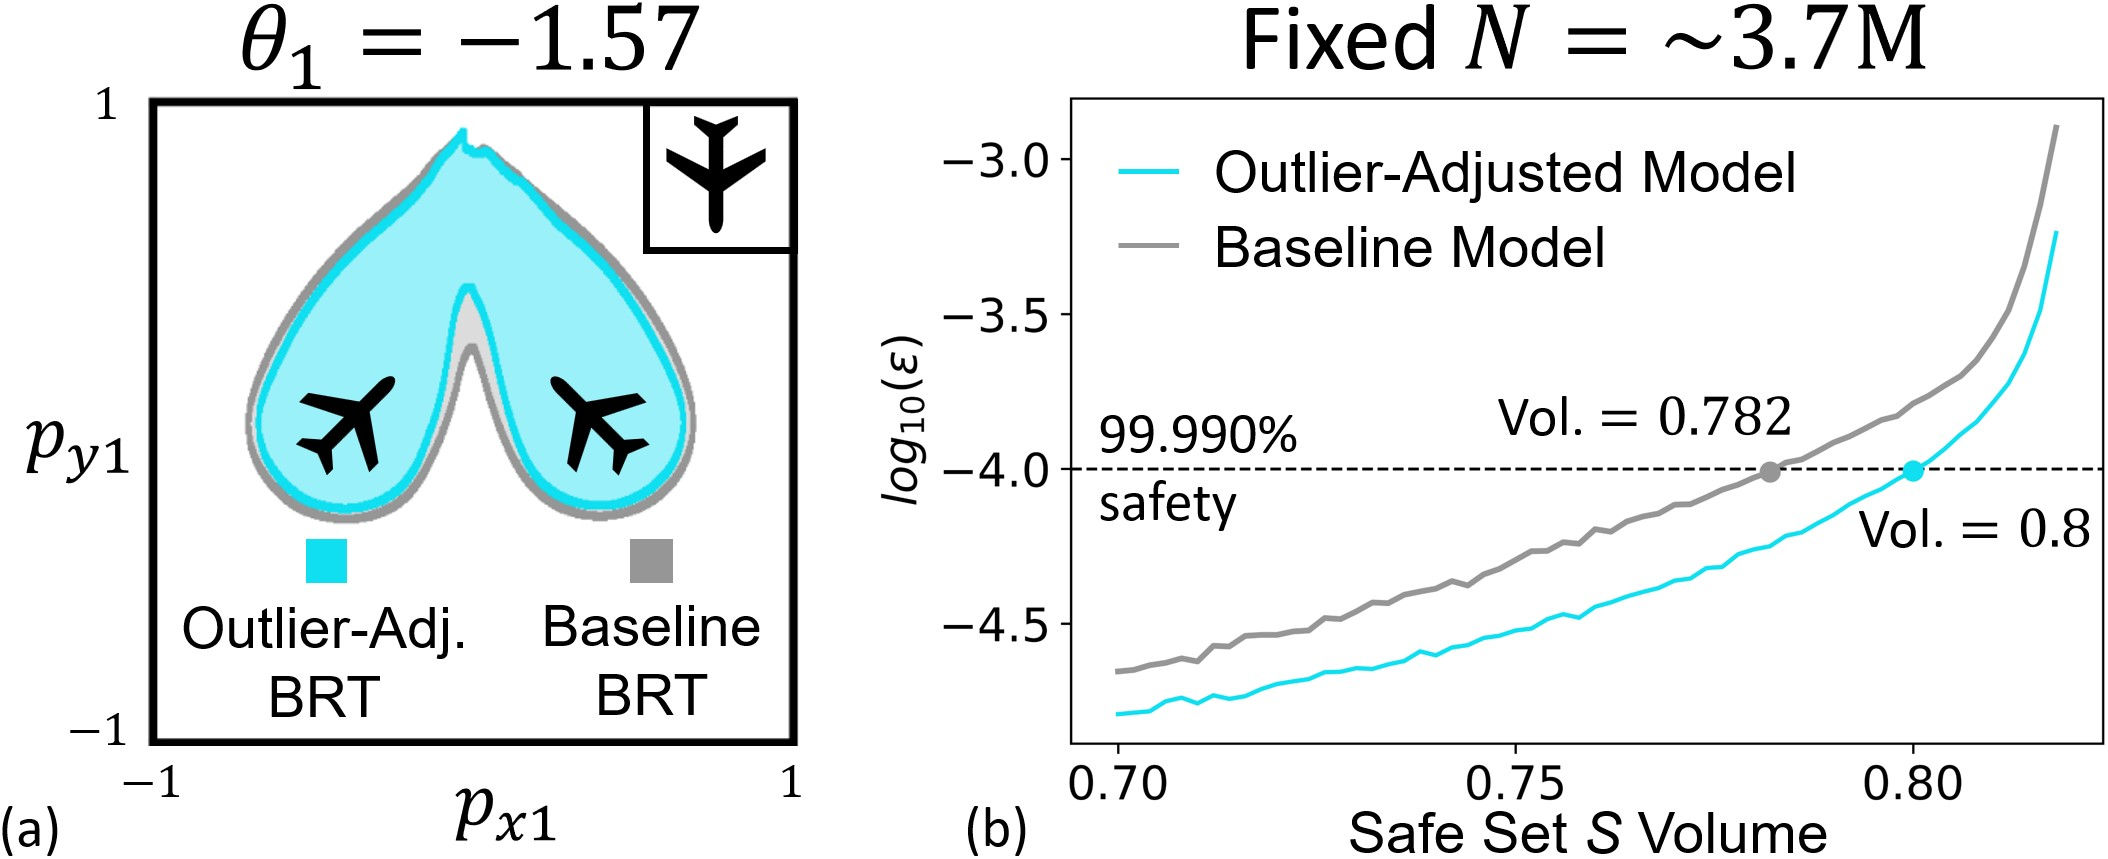
\includegraphics[width=0.6\columnwidth]{figures/Figure_3}
    \label{fig:multivehicle}
\end{SCfigure}
\vspace{-1.0em}
% 

\subsection{Rocket Landing} \label{sec:rocketlanding}
\vspace{-0.5em}
We now apply our approach to a 6D rocket landing system with position $(p_{x}, p_{y})$, heading $\theta$, velocity $(v_{x}, v_{y})$, angular velocity $\omega$, and torque controls $\tau_1, \tau_2\in [-250, 250]$. The dynamics are: $\dot{p_x} = v_x, ~\dot{p_y} = v_y, ~\dot{\theta} = \omega, ~\dot{\omega} = 0.3\tau_1, ~\dot{v_x} = \tau_1 \cos{\theta} - \tau_2 \sin{\theta}, ~\dot{v_y} = \tau_1 \sin{\theta} + \tau_2 \cos{\theta} - g$, where $g = 9.81$ is acceleration due to gravity.
The target set is the set of states where the rocket reaches a rectangular landing zone of side length 20m centered at the origin: $\targetset = \{\state: |p_x| < 20.0, p_y < 20.0\}$.
Note that we want to \textit{reach} $\targetset$, so the $\BRT$ now represents the safe set.
Results are shown in \figureref{fig:rocketlanding}.
Interestingly, a large $9.58\%$ increase in the volume of the safe set is recovered using the proposed approach, particularly near the lower-left part of the state space.
Further investigation reveals that the trajectories starting from these states exit the training regime south.
This highlights a general limitation of computing the value function over a constrained state space where information is propagated via dynamic programming, which affects both learning-based methods and traditional grid-based methods.
Nevertheless, in this case, the relative order of the value function levels is still preserved, leading to a high quality safe policy and recovery of a larger safe volume.

% 
%\vspace{-1.0em}
\begin{SCfigure}[1.22][htbp]
    \caption{Rocket Landing: outlier-adjusted (blue) and baseline (grey) results. (Left) Slice of the neural BRTs achieving $\epsilon=10^{-4}$ ($99.990\%$ safety). (Right) The outlier-adjusted approach increases the safe volume from $0.334$ to $0.366$ ($9.58\%$ increase).}
    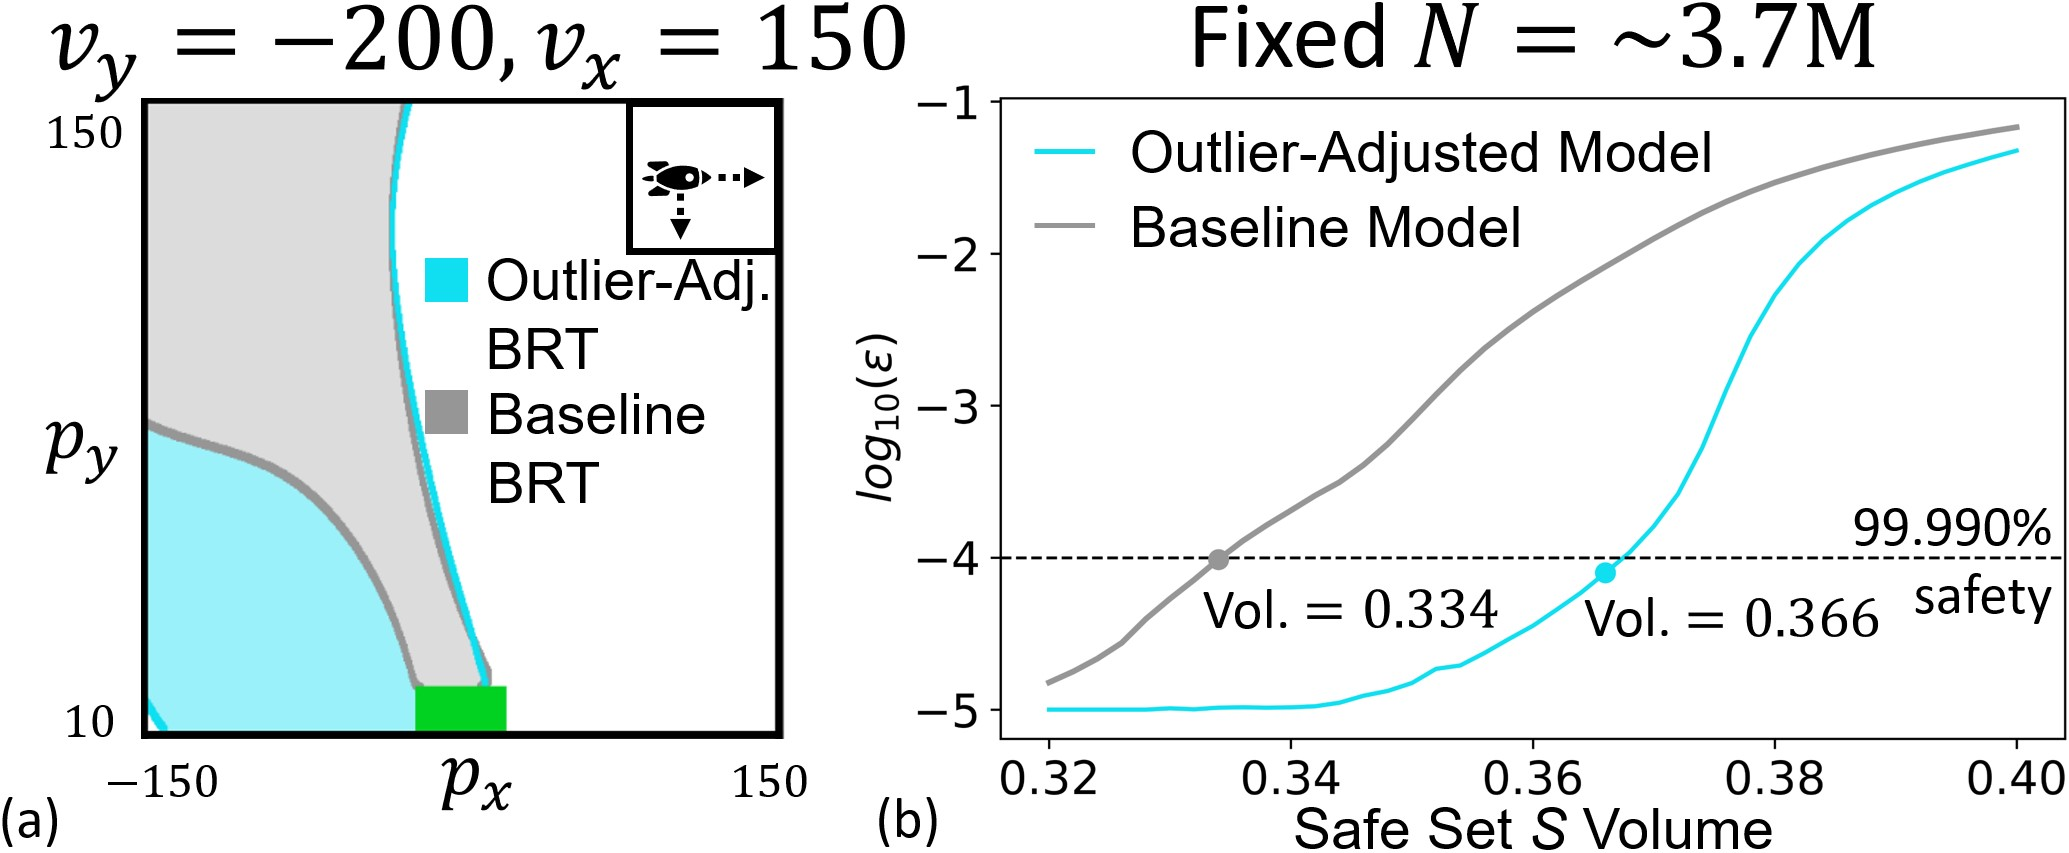
\includegraphics[width=0.6\columnwidth]{figures/Figure_4}
    \label{fig:rocketlanding}
\end{SCfigure}
%\vspace{-1.0em}
% 

\subsection{Rocket Landing with No-Go Zones} \label{sec:reachavoidrocketlanding}
\vspace{-0.5em}
We now consider the rocket landing problem in a constrained airspace where we have no-go zones of height 100m and width 10m to the left of the landing zone and where altitude is below the landing zone.
Safety in this case takes the form of a reach-avoid set - the rocket needs to reach the landing zone while avoiding the no-go zones.
An analogous HJI-VI to the one in \sectionref{sec:background_reachability} can be derived for this case, whose solution can be computed using DeepReach.
However, since reach-avoid problems are more complex than just the reach or avoid problem, the DeepReach solution results in a poor safety volume.
In fact, \textit{no} safe volume can be recovered with the desired safety level of $\epsilon \le 10^{-4}$.
In contrast, we can recover a sizable safe volume using the outlier-adjusted approach, as shown in \figureref{fig:reachavoidrocketlanding}.
These examples highlight the utility of the proposed approach.

% 
%\vspace{-1.0em}
\begin{SCfigure}[1.22][htbp]
    \caption{Rocket Landing with No-Go Zones: outlier-adjusted (blue) and baseline (grey) results. (Left) Slice of the neural BRTs achieving $\epsilon=10^{-4}$ ($99.990\%$ safety). (Right) The outlier-adjusted approach increases the safe volume from $0$ to $0.19$.}
    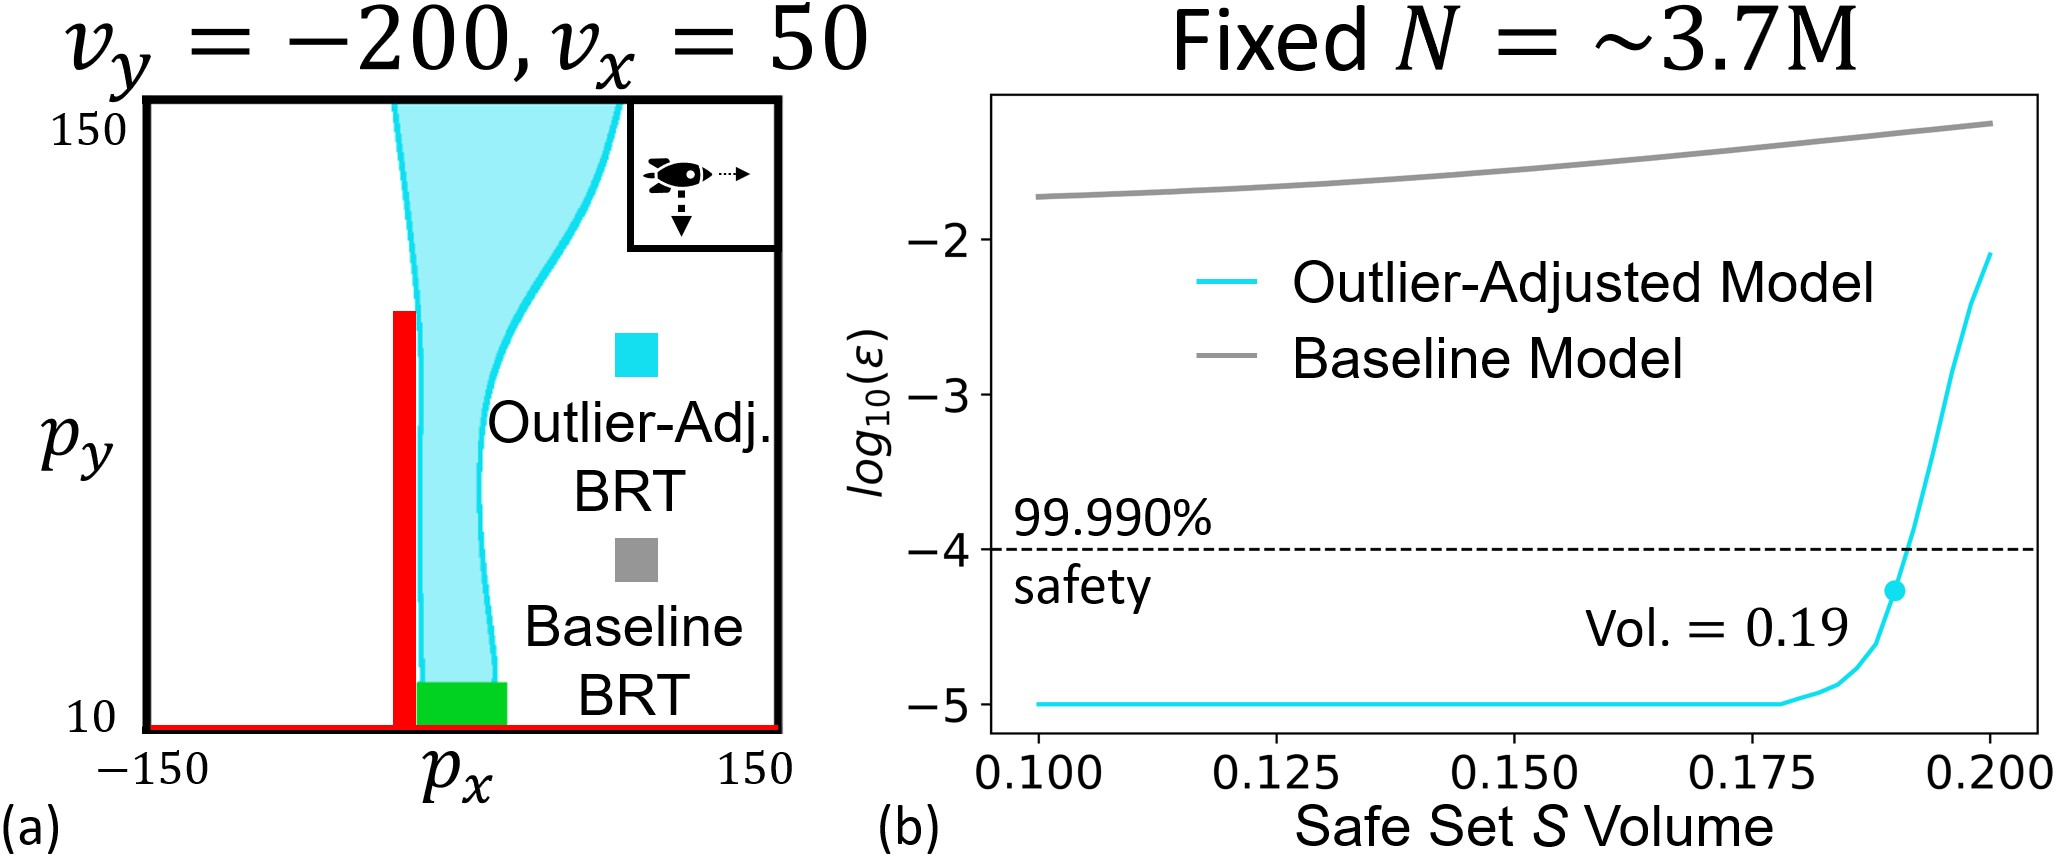
\includegraphics[width=0.6\columnwidth]{figures/Figure_5}
    \label{fig:reachavoidrocketlanding}
\end{SCfigure}
%\vspace{-1.0em}
% 